\chapter{Materials and Methods}

\section{Materials}



\begin{table}[!htb]
\caption{List of Cloning Reagents}
\rowcolors{1}{white}{black!15}
\begin{center}
\begin{tabular}{|l|l|l|}
\hline
%\multicolumn{3}{|c|}{Molecular Cloning Reagents} \\  \hline
Manufacturer & Item & Location \\ \hline \hline
\multirow{1}{*}{5 Prime} &  PerfectPrep EndoFree Plasmid Maxi Kit & \multirow{1}{*}{Gaithersburg, MD} \\
& Agarose Gelextract Mini Kit & \\ \hline
Agilent Technologies & Easy-A One-Tube RT-PCR Kit & Santa Clara, CA \\ \hline
Sigma-Aldrich & TRI Reagent\textsuperscript{\textregistered} &  Louis, MO \\ \hline
Fermentas & DNase I, RNase-free & Glen Burnie, MD \\ \hline
%Agilent Technologies & QuikChange Lightning Site-Directed Mutagenesis Kit & Santa Clara, CA \\
IBI Scientific & Ethidium Bromide (EtBr) & Peosta, IA \\ \hline
Invitrogen & MAX Efficiency\textsuperscript{\textregistered} DH10$\beta$ Competent cells & Carlsbad, CA \\ \hline
\multirow{1}{*}{Lucigen} & 2.5 mM dNTP Mix & \multirow{1}{*}{Middleton, WI} \\
& EconoTaq PLUS GREEN 2X Master Mix & \\ \hline
Promega & PureYield\textsuperscript{\texttrademark} Plasmid Miniprep System & Madison, WI \\ \hline
Research Products & Agarose & \multirow{1}{*}{Mount Prospect, IL} \\
\multirow{1}{*}{International (RPI)} & Tryptone & \\
& Yeast Extract & \\ \hline
\multirow{1}{*}{New England Biolabs} & Antarctic Phosphatase & \multirow{1}{*}{Ipswich, MA} \\
& T4 DNA Ligase & \\
& Various restriction enzymes & \\  \hline
\end{tabular}
\end{center}
\label{tab:molecular_cloning}
\end{table}%

\subsection{Restriction enzymes}
The following is a list of the restriction enzymes used. All were purchased from NEB:\begin{inparaenum}[(i)] 
\item \sali;
\item \xbai;
%\item \nrui;
\item \bamhi;
\item \stui;
\item \xhoi;
\item \apai; and
\item \kpni.
\end{inparaenum} 


\begin{table}[!htb]
\caption{List of PCR Cloning Primers}
\rowcolors{1}{white}{black!15}
\begin{center}
\begin{tabular}{|l|l|}
\hline
Primer & Sequence \\ \hline 
\hline
%\oraioneclonefwd & \salprime ATGCATCCGGAGCCCGCC \\
%\oraioneclonerev & \xbaprime CTAGGCATAGTGGCTGCCGGG \\ \hline

\oraithreeclonefwd & \salprime ATGAAGGGCGGCGAGGGG \\
\oraithreeclonerev & \xbaprime TCACACAGCCTGCAGCTCCCC \\ \hline

\stimclonefwd & \salprime ATGGATGTATGCGTCCGTC \\
\stimclonerev & \xbaprime GCCTACTTCTTAAGAGGCTTCTT \\ \hline
\end{tabular}
\end{center}
\label{tab:pcr_primers}
\end{table}%


\begin{table}[!htb]
\caption{List of RT-PCR Primers}
\rowcolors{1}{white}{black!15}
\begin{center}
\begin{tabular}{|l|l|l|}
\hline
Primer & Sequence & Size \\ \hline 
\hline
%\oraionertfwd & \ttfamily CAACTCGGTCAAGGAGTCCC & \\
%\oraionertrev & \ttfamily GTGAGCGGTAGAAGTGGACGG & \multirow{-1}{*}{311 bp} \\
%\hline
% negative multirow value is to move table entry up
% colors in table will hide multirow entry if not placed in lower cell. 
\oraithreertfwd & \ttfamily GAGTGACCACGAGTACCCACC & \\
\oraithreertrev & \ttfamily GGGTACCATGATGGCTGTGG & \multirow{-1}{*}{508 bp} \\
\hline

\stimrtfwd & \ttfamily TTGGATTCTTCCCGTTCTCACAGC & \\
\stimrtrev & \ttfamily GCCTACTTCTTAAGAGGCTTCTT & \multirow{-1}{*}{228 bp} \\ 
\hline

\rpfwd & \ttfamily ATCGGTTACGGATCGAACAA & \\
\rprev & \ttfamily GACAATCTCCTTGCGCTTCT & \multirow{-1}{*}{165 bp} \\
\hline

\hygbfwd & \ttfamily CCTGAACTCACCGCGACGTCTGTCG & \\
\hygbrev & \ttfamily AGGCAGGTCTTGCAACGTGACACC & \multirow{-1}{*}{303 bp} \\ 
\hline
\end{tabular}
\end{center}
\label{tab:rtpcr_primers}
\end{table}%


\subsection{Primers}
All primers were purchased from Integrated DNA Technologies (Coralville, IA).

\begin{table}[!htb]
\caption{List of Cell Culture Reagents}
\rowcolors{1}{white}{black!15}
\begin{center}
\begin{tabular}{|l|l|l|}
\hline
%\multicolumn{3}{|c|}{Cell Culture Reagents} \\ \hline
Manufacturer & Item & Location \\  \hline \hline
Atlanta Biologicals & Fetal Bovine Serum - catalog no. S11050 & Lawrenceville, GA \\ \hline
Lonza & Schneider's Drosophila Medium & Walkersville, MD \\ \hline
%RPI & Hygromycin B & \multirow{1}{*}{Mount Prospect, IL} \\ \hline
\end{tabular}
\end{center}
\label{tab:cell_culture}
\end{table}%

\subsection{\droso{} resources}
\droso{} Schneider line 2 (S2) cells, the \puchygmt{} plasmid and the  {puc18-act-gfp} plasmid were all purchased from the Drosophila Genomics Resource Center (Bloomington, IN). Figure~\ref{fig:puchyg_map} shows a schematic of the \puchygmt{} vector, with possible sites of insertion in the multiple cloning site (MCS). 
%\todo{check if quikchange and other cloning entries relevant}



\begin{figure}[!h]
\begin{center}
	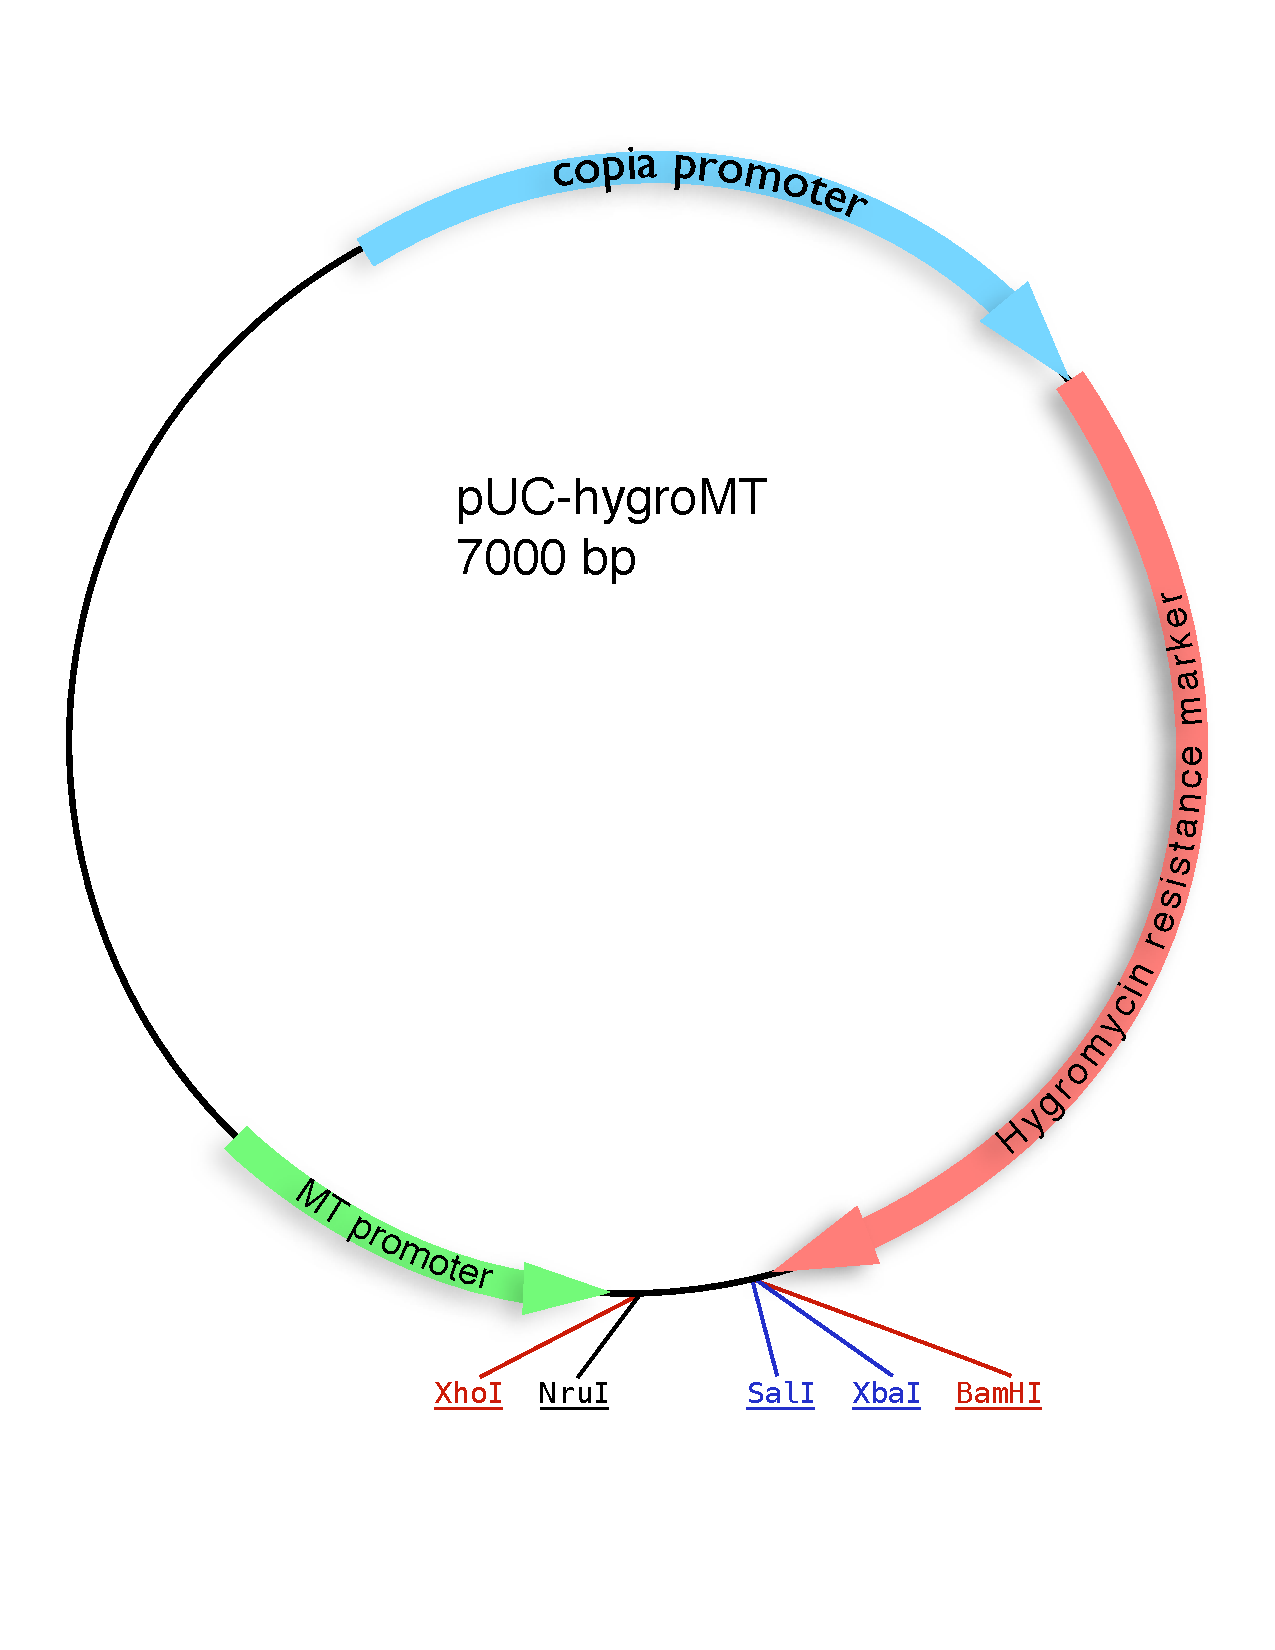
\includegraphics[scale=0.58]{Figures/puchygromt.pdf}\vspace{-45pt}

	\caption[Map of the puc-HygroMT vector]{{\bfseries Map of the \puchygmt{} vector.} \puchygmt{} contains \sali{} and \xbai{} sites which were used to insert both Orai3 and STIM1 into the MCS.}
	\label{fig:puchyg_map}

\end{center}
\end{figure}

 

\begin{table}[!htb]
\caption{List of Chemical Reagents}
\rowcolors{1}{white}{black!15}
\begin{center}
\begin{tabular}{|l|l|l|}
\hline
%\multicolumn{3}{|c|}{Chemicals} \\ \hline 
Manufacturer & Item & Location \\ \hline  \hline
Acros Organics &  Ethylene Glycol Tetraacetic Acid (EGTA) & Geel, Belgium \\
& 4-(2-hydroxyethyl)-1-piperazineethanesulfonic & \\
& acid (HEPES) & \\
& HEPES Sodium Salt (HEPES-Na) & \\
& Paraformaldehyde 96\% & \\
& Sodium Chloride (NaCl) & \\ \hline
Fisher Scientific & Cupric Sulfate Pentahydrate (\CuSO) & Fair Lawn, NJ \\
& Dimethyl Sulfoxide (DMSO) & \\
& D-glucose & \\
& Hydrochloric Acid (HCl) 10N & \\
& Potassium Chloride (KCl) & \\
& Sodium Hydroxide (NaOH) 10N & \\ \hline
Invitrogen & Fura-2 AM & Carlsbad, CA \\ \hline
Mirus Bio LLC & \transit Transfection Reagent & Madison, WI \\ \hline
\multirow{1}{*}{MP Biomedicals} & Agar & \multirow{1}{*}{Solon, OH} \\
& Probenecid & \\ \hline
\multirow{1}{*}{Sigma-Aldrich} & 2-Aminoethyl diphenylborinate (2-APB) & \multirow{1}{*}{St. Louis, MO} \\
& Cyclopiazonic Acid (CPA) & \\
& \Pluronic & \\
& Fluka Analytical 1.0 M \CaCl & \\
& Fluka Analytical 1.0 M \MgCl & \\ \hline
\end{tabular}
\end{center}
\label{tab:chemical_reagents}
\end{table}%



\begin{table}[!htb]
\caption{List of Instruments}
\rowcolors{1}{white}{black!15}
\begin{center}
\begin{tabular}{|l|l|l|}
\hline
%\multicolumn{3}{|c|}{Instruments} \\ \hline 
Manufacturer & Item & Location \\ \hline \hline
Applied Biosystems & 2720 Thermal Cycler & Foster City, CA \\ \hline
Denver Instruments & UltraBasic pH/mV meter & Bohemia, NY \\ \hline
Sutter Instrument & Lambda 10-B & Novato, CA \\ \hline
Thermo Fisher Scientific & NanoDrop ND 1000 & Wilmington, DE \\ \hline
Intracellular Imaging Inc. & 175 W Xenon Lamp & Cincinnati, OH \\ \hline
B \& B Microscopes, Ltd. & Olympus CKX41 Inverted Microscope & Pittsburgh, PA \\ \hline 
\end{tabular}
\end{center}
\label{tab:instruments}
\end{table}% 

\section{Methods}

\subsection{Maintenance of cell lines}
\droso{} S2 cells were cultured at 27 \textcelsius{} in Schneider's \droso{} medium supplemented with 10\% fetal bovine serum (FBS). 

\subsection{Creation of \droso{} expression constructs}

\subsubsection{Molecular Cloning}
%Orai1, 
We needed to express human genes (Orai3, Stim1) on a \droso{} background, a process which required some molecular biology finesse. We chose to accomplish this by transferring these genes to a \droso{} vector.  We selected the \puchygmt{} plasmid as our vector, whereas Orai3 and Stim1 were the kind gifts of Dr. Stefan Feske, NYU School of Medicine.

\puchygmt{}  (see figure~\ref{fig:puchyg_map}) contains a metallothionein promoter %(17.)
 before the MCS, allowing one to induce the expression of genes placed in the MCS. It  provides the necessary genes for driving constitutive hygromycin B resistance %(17.)
%. Also, \puchygmt{} was available at a significantly lower cost compared to alternative vectors from commercial suppliers. Additionally, 
 and, the use of this vector for induction and creation of stable lines has previously been documented \citep{Eble1998}. 

Our genes of interest -- human %Orai1, 
Orai3 and STIM1 -- were ligated into the \puchygmt{} plasmid using \sali{} and \xbai{} sites. The inserts for our genes of interest were created by polymerase chain reaction (PCR) using the primers listed in Table~\ref{tab:pcr_primers}. 
%The \oraioneclonefwd and \oraioneclonerev  primer pair were used for the Orai1 insert. 
The \oraithreeclonefwd and \oraithreeclonerev primers were used for the Orai3 insert. 
The Stim1 insert was generated using \stimclonefwd and \stimclonerev  primers. 
The forward primer for each insert contained a \sali{} restriction site (\salisite), protected by the \nruisite{} sequence. The reverse primer for each insert had an \xbai{} restriction site (\xbaisite), protected by the \nruisite{} sequence. 

Each PCR reaction consisted of: 
\begin{inparaenum}[(i)] 
\item 1X Easy-A reaction buffer;
\item .2 mM dNTPs;
\item 2 $\mu$M forward; and
\item 2 $\mu$M reverse primers; 
\item 2 $\mu$L Easy-A PCR enzyme; 
\item 50-100 ng of template DNA; and
\item nuclease-free water up to 100 $\mu$L. 
%\item 10\% DMSO was also added to the Orai1 PCR reaction.
\end{inparaenum}

The PCR reaction thermocycler parameters for each amplicon were as follows: 

\textbf{\itshape %Orai1 and 
Orai3}, 
\begin{inparaenum}[(i)]
\item an initial denaturation step at 95 \textcelsius{} for 3 minutes;
\item 27 cycles of denaturation at 95 \textcelsius{} for 40 seconds, followed by annealing at 65 \textcelsius{} for 30 seconds, then extension at 72 \textcelsius{} for 1 minute; and
\item a final extension of 72 \textcelsius{} for 7 minutes. 
\end{inparaenum}

\textbf{\itshape STIM1}, 
\begin{inparaenum}[(i)]
\item an initial denaturation step at 95 \textcelsius{} for 3 minutes;
\item 27 cycles of denaturation at 95 \textcelsius{} for 40 seconds, followed by an annealing step at 65 \textcelsius{} for 30 seconds, then extension at 72 \textcelsius{} for 130 seconds; and
\item a final extension of 72 \textcelsius{} for 7 minutes were performed. 
\end{inparaenum}

After the PCR reactions were completed, the amplicons were digested with \sali{} and \xbai, then ligated into a similarly digested \puchygmt{} vector (see details below).

\subsubsection{Engineering \droso{} vector contructs}
Each PCR product and the \puchygmt{} vector were digested by \sali{} and \xbai{} restriction enzymes. The vector digest was followed by treatment with Antarctic Phosphatase, according to the manufacturer's instructions. Phosphatase treatment removed the 5$^\prime$ phosphate group at the end of the digested vector DNA. This helped prevent spontaneous recircularization and increased the amount of vector available to ligate with the insert. The digested vector and digested PCR amplicons were run on a 0.8\% 1X TAE agarose gel for 90 minutes at 80 V. Following electrophoresis, the DNA band was excised under UV illumination. The vector and insert DNA were then purified using the Agarose GelExtract Mini kit. After purifying the DNA, a ligation reaction was performed with T4 DNA ligase following the manufacturer's specifications. The insert to vector ratios in the ligations were 9:1 (by volume). After a 15 minute incubation at 25 \textcelsius{}, the ligation mixture was used to transform DH10$\beta$ competent cells. The ligated constructs were renamed to indicate the inserts, thus %\oraiivector{} contained Orai1,
\underline{\oraiiiivector{}} contained Orai3, while \underline{\stimivector{}} contained Stim1.

\subsubsection{Transformation of ligated DNA}
A 15 ml round-bottom tube was chilled on ice, prior to addition of 100 $\mu$L thawed DH10$\beta$ cells. Subsequently, 4 $\mu$L of the ligation mixture was added, mixed gently by flicking, then chilled on ice for 30 minutes. Next, the tube was incubated at 42 \textcelsius{} for 45 seconds, then quickly transferred to ice for 90 seconds. After this, 900 $\mu$L of SOC medium was added. A one hour incubation at 37 \textcelsius{} followed, with shaking at 250 RPM. 200 $\mu$L of this transformation mixture was plated on LB-Agar plates containing 100 $\mu$g/mL of the antibiotic ampicillin (+Amp). The resulting LB-Agar +Amp plates were placed in an incubator at 37 \textcelsius{} overnight. After 16-18 hrs the plates were transferred to 4 \textcelsius{}. Individual colonies from these plates were used to start miniprep cultures and obtain plasmid DNA.

\subsubsection{Minipreparation of plasmid DNA}
Single colonies were picked and added to 4 ml of LB supplemented with 100 $\mu$g/mL of ampicillin. This mixture was placed in an incubator at 37 \textcelsius{}, with shaking at 250 rpm, for 16-18 hours. A miniprep procedure was performed according to the instructions provided with the Pureyield\textsuperscript{\texttrademark} Plasmid Miniprep System. DNA concentrations were estimated using a NanoDrop ND 1000 spectrophotometer.

\subsubsection{Maxipreparation of plasmid DNA}
A maxiprep culture consisting of 100 ml of LB, supplemented with 100 $\mu$g/ml of ampicillin was started, using 100 $\mu$L of the miniprep culture. This mixture was placed in an incubator at 37 \textcelsius{}, with shaking at 250 rpm, for 16-18 hours. A maxiprep procedure was performed according to the protocol of the PerfectPrep EndoFree Plasmid Maxi kit. DNA concentrations were estimated using a NanoDrop ND 1000 spectrophotometer.


\subsection{Transfection of S2 cells}
S2 cells were transfected with \transit transfection reagent according to the manufacturer's instructions. Briefly, one day prior to transfection, S2 cells were plated at 80\% confluency in a 6-well tissue culture plate. \oraiiiivector{} vector transfections were done with 1 $\mu$g of DNA per well. Transfections involving \stimivector{} used 2 $\mu$g of DNA per well. \stimivector{} and \oraiiiivector{} co-transfections were performed at a 2:1 ratio (Stim1:Orai3). 

As a positive control for transfection, 0.25 $\mu$g of the green fluorescent protein (GFP) vector \pucgfp, was co-transfected with the above constructs. A ratio of 3 $\mu$L of \transit was used per 1 $\mu$g of maxiprepped DNA.

\subsubsection{Induction of transfected S2 cells with \cuso}
\droso{} S2 cells were induced by the addition of 750 $\mu$M \cuso{} one or two days post-transfection.

\subsection{RT-PCR and cDNA synthesis} %http://www.ncbi.nlm.nih.gov/pmc/articles/PMC2717784/
%Briefly, an aliquot of 1± 1.5 mg cell protein was incubated in 500 ml buffer alone (control) or supplemented with various inhibitors, and incubation took place for 30 min at 37VC under an atmosphere of 95\% oxygen and 5\% carbon dioxide. Subsequently, the samples were centrifuged for 3 min at 100 Tg and 4VC, and 100 ml 3 N perchloric acid was added to the pellet, which was then vortex- mixed, let 5 min to rest, again vortexed and centrifuged for 3 min at 100Tg. The sample was neutralized with 125 ml medium containing 2 N KOH, 0.4 M imidazole and 0.4 M KCl, vortex-mixed and centrifuged again.
Total RNA was isolated from transfected S2 cells, two days post-induction, using TRI reagent\textsuperscript{\textregistered} as per the manufacturer's instructions. 
% Transfected, induced S2 cells were removed from a 100 mm dish by repeated pipetting with a serological pipet. This was followed by collecting the cells via centrifugation at 200 x g for 3 minutes. The old media was aspirated from the cells and then dissolved in 1 ml of TRI reagent\textsuperscript{\textregistered}. Two 100 mm dishes were used per transfection. The TRI reagent\textsuperscript{\textregistered} and dissolved cell mixture had 200 $\mu$L of chlorform added. This was shaken vigrously for 30 seconds, then left standing at room temperature for 15 minutes. All centrifugation spins were performed at 4 \textcelsius{}. A spin at 12000 x g for 15 minutes followed. The colorless, aqueous phase was removed and 750 $\mu$L of isopropanol added. After shaking this mixture was incubated at room temperature for 10 minutes, then spun at 12000 x g for 10 minutes. The supernatant was removed leaving behind a pellet. This pellet was washed with 75\% Ethanol, and then centrifuged again for 10 minutes at 7500 x g. The supernatant was again removed and the remaining pellet was allowed to air-dry at room temperature for 10 minutes. The pellet containing RNA was then resuspended in 40-50 $\mu$L of nuclease-free water. The RNA concentration was then determined using a NanoDrop ND 1000 spectrophotometer.
Traces of contaminating DNA were removed using RNase-free DNase I. 
For each $\mu$g of RNA, 1 $\mu$L of DNase I was added. First strand cDNA synthesis was performed using the MMLV reverse transcriptase (RT). Briefly, 1 $\mu$g of mRNA was reverse transcribed into cDNA during a 30 minute incubation at 45 \textcelsius{}. This cDNA served as the template for successive PCR reactions. 


The RT reaction mixture contained:
\begin{inparaenum}[(i)] 
\item 1X MMLV buffer;
\item .8 mM dNTPs; 
\item 1 $\mu$g of template RNA; 
\item 2 $\mu$L MMLV RT; and
\item nuclease-free water up to 50 $\mu$L. 
RT reactions were also performed on samples with the RT omitted -- to determine whether any contaminating DNA was still present. 
\end{inparaenum}

PCR reactions were performed in a 2720 Thermal Cycler. The \droso{} housekeeping gene, ribosomal protein 49 (rp49), was used as a positive control to determine whether cDNA was made in the preceding RT reaction \citep{Bunch1988, Luce-Fedrow2008}.


Each PCR reaction contained:
\begin{inparaenum}[(i)] 
\item 1X Easy-A reaction buffer;
\item .3 mM dNTPs;
\item 1 $\mu$M forward; and
\item 1 $\mu$M reverse primers; 
\item .5 $\mu$L Easy-A PCR enzyme; 
\item 5 $\mu$L of cDNA template from the (no-)RT reaction; and
\item nuclease-free water up to 50 $\mu$L. The sequences of these RT-PCR primers \citep{Luce-Fedrow2008, Mignen2008a, Xu2010}, and expected band sizes are given in Table \ref{tab:rtpcr_primers}.
\end{inparaenum}

The PCR reaction parameters are as follows: 

\textbf{\itshape
Orai3 and STIM1},
\begin{inparaenum}[(i)]
\item an initial denaturation step at 95 \textcelsius{} for 3 minutes;
\item 30 cycles of denaturation at 95 \textcelsius{} for 30 seconds, then annealing at 55 \textcelsius{} for 30 seconds, then extension at 72 \textcelsius{} for 1 minute; and
\item a final extension of 72 \textcelsius{} for 10 minutes was performed. 
\end{inparaenum}

\textbf{\itshape HygBP}, 
\begin{inparaenum}[(i)]
\item an initial denaturation step at 95 \textcelsius{} for 3 minutes;
\item 30 cycles of denaturation at 95 \textcelsius{} for 30 seconds, then annealing at 65 \textcelsius{} for 30 seconds, then extension at 72 \textcelsius{} for 30 seconds; and
\item a final extension of 72 \textcelsius{} for 10 minutes was performed. 
\end{inparaenum}

\textbf{\itshape rp49}, 
\begin{inparaenum}[(i)]
\item an initial denaturation step at 94 \textcelsius{} for 3 minutes;
\item 30 cycles of denaturation at 94 \textcelsius{} for 45 seconds, then annealing at 50 \textcelsius{} for 1 minute, then extension at 72 \textcelsius{} for 1 minute 30 seconds; and
\item a final extension of 72 \textcelsius{} for 7 minutes was performed. 
\end{inparaenum}

%RT-PCR products were viewed electrophoretically on 0.8% agarose gels stained with ethidium bromide. Gels were viewed on the LAS 4000 imaging system.

%\subsection{Microscopy Imaging}
%GFP transfected S2 cells were fixed with 2\% paraformaldehyde prior to viewing on a \todo{insert EPI microscope name and manufacturer here}. 
%A poly-D lysine treated microscope slide was outlined with a Pap Pen, \todo{cite Pap Pen info} and GFP transfected S2 cells were allowed to attach for 4 hours. The media was removed, and the attached S2 cells rinsed in 1x PBS. The cells were fixed with 2\% paraformaldehyde for 10 minutes, then rinsed twice with 1x PBS. A drop of Vectashield was placed in the middle of the slide, and the glass coverslip applied afterwards. Images were then taken with a FITC filter on the EPI scope \todo{insert EPI microscope name and manufacturer here}


\subsection{Ca$^{2+}$ imaging experiments}
Two primary solutions were used for the \Ca{} imaging experiments. The first, designated \textbf{2 Ca}, contained (in mM): 2 \CaCl, 4 \MgCl, 150 NaCl, 5 KCl, 10 HEPES and, 10 D-glucose at pH 7.2 \citep{Zhang2005}. The second solution \textbf{1 EGTA}, contained (in mM), 1 EGTA, 6 \MgCl, 150 NaCl, 5 KCl, 10 HEPES and, 10 D-glucose at pH 7.2 \citep{Zhang2005}. The dye loading solution referred to below was comprised of 2 Ca, 0.02\% Pluronic F-127, 2.5 mM probenecid and 4 $\mu$M Fura2-AM. %\todo{mention that this composition was primarily from the Kozak/Stim1 paper in intro}


Cytosolic \Ca{} signals were measured in the following way: S2 cells, cultured at 27 \textcelsius{}, were plated on 35 mm glass-bottom chambers made by J. Ashot Kozak, Ph. D. The cells were allowed to adhere for 30 minutes at room temperature, the old medium was removed, and the cells washed in 1X DPBS twice. After the wash, the dye-loading solution was added to the attached cells and they were incubated at room temperature for 45 minutes. The cells were then washed twice with the 2 Ca solution, and used for imaging. 

\Ca{} imaging was performed on the stage of an Olympus CKX41 inverted microscope. Cells were perfused at a rate of approximately 4 mL/min using the solutions indicated in the figures below. Loaded cells were exposed to light of 340 nm and 380 nm wavelengths, and emitted light at 510 nm was recorded by the InCytIM 2 imaging system (Intracellular Imaging, Cincinnati, OH) installed on a Dell Optiplex 745C computer. The UV light source was a 175 W Xenon arc lamp. The wavelengths were selected using filters in the Lambda 10-B SmartShutter which was controlled by the InCytIM 2 software. 


\subsubsection{Selection of data for analysis}
The traces were selected based on the following criteria: 
\begin{inparaenum}[(i)]
\item there was a visible response to CPA introduction; 
\item the initial perfusion with 2 Ca was relatively stable over time;
\item the absolute values of the measurements at 340 nm and 380 nm were $\ge$ 40 during initial perfusion with 2 Ca; and
\item the 340 nm and 380 nm recordings mirrored each other as time progressed.
\end{inparaenum}

\subsubsection{Statistical analysis of imaging experiment data}
Error bars shown on the traces depict the standard error of the mean. Area under the curve analysis was performed using Origin 8 software. Statistical analysis of the area under the curve data was performed using one way ANOVA with SAS software. 
% Check this sentence for ERRORS
Differences were considered significant if p values were $<$ 0.05. The p values of $<$ 0.0001 were denoted by the *** characters.

% -eof-
